\documentclass[10pt, aspectratio=169]{beamer}

% Theme Selection
\usetheme{Madrid}
\usecolortheme{seahorse}

% Packages
\usepackage{amsmath, amssymb, amsfonts}
\usepackage{graphicx}
\usepackage{booktabs}
\usepackage{multicol}
\usepackage{url}
\usepackage{tikz}
\usepackage{pgfplots}
\pgfplotsset{compat=1.18}

% Presentation Metadata
\title[Module 3: Descriptive Statistics]{Mathematics for Computing}
\subtitle{A Report on Official Statistical Machinery \& Module 3: Descriptive Statistics}
\author{Alen Francis Joseph}
\institute{M.Tech CSE (DS and AI), DCS, CUSAT}
\date{\today}

\begin{document}

% -----------------------------------------------------------------------------
% Title Slide
% -----------------------------------------------------------------------------
\begin{frame}
    \titlepage
\end{frame}

% -----------------------------------------------------------------------------
% Table of Contents
% -----------------------------------------------------------------------------
\begin{frame}{Module Outline}
    \tableofcontents
\end{frame}

% =============================================================================
\section{Official Statistical System (Govt. of India \& Kerala)}
% =============================================================================

\begin{frame}{Ministry of Statistics \& Programme Implementation (MoSPI)}
    \begin{block}{Overview \& Mission}
        MoSPI is the apex executive body responsible for the development, coverage, quality, and dissemination of official statistics in India, as well as monitoring major national development projects.
    \end{block}

    \begin{columns}[T]
        \begin{column}{0.48\textwidth}
            \textbf{1. Statistics Wing (NSO)}
            \begin{itemize}
                \item \textbf{Central Statistical Office (CSO):} Coordinates statistical activities, National Accounts (GDP), Industrial Statistics.
                \item \textbf{National Sample Survey Office (NSSO):} Conducts large-scale socio-economic sample surveys nationwide.
            \end{itemize}
        \end{column}
        
        \begin{column}{0.48\textwidth}
            \textbf{2. Programme Implementation Wing}
            \begin{itemize}
                \item \textbf{Infrastructure Monitoring:} Tracks Central Sector Projects ($>$ Rs.150 Crore).
                \item \textbf{Twenty Point Programme (TPP):} Monitors key poverty alleviation schemes.
                \item \textbf{MPLADS:} Oversees the MP Local Area Development Scheme.
            \end{itemize}
        \end{column}
    \end{columns}
\end{frame}

\begin{frame}{Department of Economics \& Statistics (DES), Govt. of Kerala}
    \begin{block}{Overview \& Organizational Structure}
        DES Kerala is the state's nodal agency responsible for the systematic collection, compilation, analysis, and dissemination of official statistics for evidence-based governance and state planning.
    \end{block}

    \begin{block}{Administrative Hierarchy}
        \begin{itemize}
            \item \textbf{Headquarters (Directorate):} Vikas Bhavan, Thiruvananthapuram.
            \item \textbf{District Level:} 14 District Offices, each headed by a Deputy Director.
            \item \textbf{Sub-District / Field Level:} 61 Taluk Statistical Offices managing data collection across Municipalities and Panchayaths.
        \end{itemize}
    \end{block}
\end{frame}

% =============================================================================
\section{Introduction to Descriptive Statistics}
% =============================================================================

\begin{frame}{Overview of Descriptive Statistics}
    \begin{block}{What is Descriptive Statistics?}
        Descriptive statistics involves summarizing, organizing, and presenting data in a meaningful way using numerical measures, tables, and graphical displays.
    \end{block}

    \vspace{0.2cm}
    \begin{columns}[T]
        \begin{column}{0.48\textwidth}
            \textbf{Descriptive Statistics}
            \begin{itemize}
                \item Focuses on summarizing observed sample data.
                \item Uses measures of central tendency and dispersion.
            \end{itemize}
        \end{column}
        
        \begin{column}{0.48\textwidth}
            \textbf{Inferential Statistics}
            \begin{itemize}
                \item Makes predictions about a population based on a sample.
                \item Uses probability models.
            \end{itemize}
        \end{column}
    \end{columns}

    \begin{exampleblock}{Example: Descriptive vs Inferential}
        \textbf{Descriptive:} The average score of 50 students in this class is 78\%. \\
        \textbf{Inferential:} Based on this class's sample average, we estimate with 95\% confidence that the average score of all 500 students in the university is between 75\% and 81\%.
    \end{exampleblock}
\end{frame}

% =============================================================================
\section{Histograms}
% =============================================================================

\begin{frame}{Histograms}
    \begin{definition}[Histogram]
        A \textbf{histogram} is an approximate representation of the distribution of numerical data. It partitions the spread of the data into contiguous intervals called \textbf{bins}.
    \end{definition}

    \begin{columns}[c]
        \begin{column}{0.52\textwidth}
            \begin{exampleblock}{Example: Constructing a Histogram}
                \textbf{Data (Ages):} $22, 23, 24, 25, 25, 26, 28, 29$ \\
                \textbf{Bins:} $[21-23], [24-26], [27-29]$
                \begin{itemize}
                    \item Bin $[21-23]$: Contains $22, 23$ (\textbf{Freq = 2})
                    \item Bin $[24-26]$: Contains $24, 25, 25, 26$ (\textbf{Freq = 4})
                    \item Bin $[27-29]$: Contains $28, 29$ (\textbf{Freq = 2})
                \end{itemize}
            \end{exampleblock}
        \end{column}
        
        \begin{column}{0.45\textwidth}
            \centering
            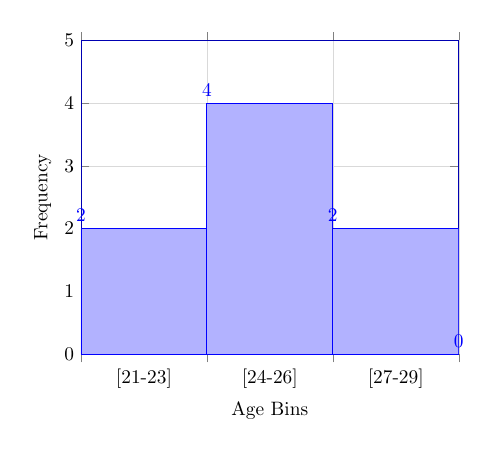
\begin{tikzpicture}[scale=0.7]
                \begin{axis}[
                    ybar interval,
                    ymin=0, ymax=5,
                    xmin=21, xmax=30,
                    xlabel={Age Bins},
                    ylabel={Frequency},
                    xtick={21, 24, 27, 30},
                    xticklabels={[21-23], [24-26], [27-29], },
                    ytick={0, 1, 2, 3, 4, 5},
                    grid=both,
                    major grid style={line width=.2pt,draw=gray!30},
                    nodes near coords,
                    nodes near coords align={vertical},
                    fill=blue!30,
                    draw=blue!70!black
                ]
                    \addplot coordinates { (21,2) (24,4) (27,2) (30,0) };
                \end{axis}
            \end{tikzpicture}
        \end{column}
    \end{columns}
\end{frame}

% =============================================================================
\section{Sample Mean and Sample Variance}
% =============================================================================

\begin{frame}{Sample Mean, Variance and Standard Deviation}
    \begin{definition}[Sample Mean and Variance]
        $$\bar{x} = \frac{1}{n} \sum_{i=1}^{n} x_i \quad \text{and} \quad s^2 = \frac{1}{n-1} \sum_{i=1}^{n} (x_i - \bar{x})^2$$
    \end{definition}

    \begin{exampleblock}{Example: Calculating Mean and Variance}
        \textbf{Data:} $2, 4, 6$ (Sample size $n=3$) \\
        \textbf{Mean ($\bar{x}$):}
        $$\bar{x} = \frac{2 + 4 + 6}{3} = \frac{12}{3} = 4$$
        \textbf{Variance ($s^2$):} 
        $$s^2 = \frac{(2-4)^2 + (4-4)^2 + (6-4)^2}{3-1} = \frac{(-2)^2 + 0^2 + 2^2}{2} = \frac{4 + 0 + 4}{2} = 4$$
        \textbf{Standard Deviation ($s$):} $\sqrt{4} = 2$.
    \end{exampleblock}
\end{frame}

% =============================================================================
\section{Order Statistics}
% =============================================================================

\begin{frame}{Order Statistics}
    \begin{definition}[Order Statistics]
        When sample observations $x_1, x_2, \dots, x_n$ are arranged in ascending order, the resulting ordered values $x_{(1)} \le x_{(2)} \le \dots \le x_{(n)}$ are known as order statistics.
    \end{definition}

    \begin{exampleblock}{Example: Finding Order Statistics}
        \textbf{Raw Data:} $12, 7, 9, 3, 15$ \\
        \textbf{Ordered Data:} $3, 7, 9, 12, 15$ ($n=5$)
        \begin{itemize}
            \item \textbf{1st Order Statistic (Minimum):} $x_{(1)} = 3$
            \item \textbf{5th Order Statistic (Maximum):} $x_{(5)} = 15$
            \item \textbf{Median (Middle value, $x_{(3)}$):} $9$
            \item \textbf{Range:} $x_{(5)} - x_{(1)} = 15 - 3 = 12$
        \end{itemize}
    \end{exampleblock}
\end{frame}

% =============================================================================
\section{Sample Covariance \& Covariance Matrix}
% =============================================================================

\begin{frame}{Sample Covariance and Covariance Matrix}
    \begin{definition}[Sample Covariance]
        $$s_{xy} = \frac{1}{n-1} \sum_{i=1}^{n} (x_i - \bar{x})(y_i - \bar{y})$$
    \end{definition}

    \begin{definition}[Sample Covariance Matrix]
        For a dataset with $p$ variables, the sample covariance matrix $S$ is a $p \times p$ symmetric matrix where the diagonal elements are variances and off-diagonals are covariances:
        $$S = \frac{1}{n-1} \sum_{i=1}^{n} (\mathbf{x}_i - \bar{\mathbf{x}})(\mathbf{x}_i - \bar{\mathbf{x}})^T$$
    \end{definition}
\end{frame}

\begin{frame}{Example: Covariance and Covariance Matrix}
    \begin{exampleblock}{Example: Calculating Covariance}
        \textbf{Data:} $X = (1, 2, 3)$, $Y = (2, 4, 6)$ \\
        \textbf{Means:} $\bar{x} = 2$, $\bar{y} = 4$ \\
        \textbf{Covariance ($s_{xy}$):}
        $$s_{xy} = \frac{(1-2)(2-4) + (2-2)(4-4) + (3-2)(6-4)}{3-1} = \frac{(-1)(-2) + 0 + (1)(2)}{2} = \frac{4}{2} = 2$$
    \end{exampleblock}

    \begin{exampleblock}{Example: Constructing the Matrix}
        With $s_x^2 = 1$, $s_y^2 = 4$, and $s_{xy} = 2$, the $2 \times 2$ covariance matrix is:
        $$S = \begin{pmatrix} s_x^2 & s_{xy} \\ s_{xy} & s_y^2 \end{pmatrix} = \begin{pmatrix} 1 & 2 \\ 2 & 4 \end{pmatrix}$$
    \end{exampleblock}
\end{frame}

% =============================================================================
\section{Frequentist Statistics}
% =============================================================================

\begin{frame}{Frequentist Statistics: Sampling}
    \begin{block}{Frequentist Paradigm}
        Frequentist statistics views probability as the long-run frequency of events. True population parameters (e.g., mean $\mu$) are considered \textbf{fixed but unknown}, and sample data are treated as random outcomes from repeated experiments.
    \end{block}

    \begin{block}{Sampling}
        Drawing a subset of data from the population to estimate parameters. The estimators themselves are random variables with their own sampling distributions.
    \end{block}

    \begin{exampleblock}{Example: Sampling Distribution}
        If you repeatedly draw samples of size $n=30$ from a population and compute the sample mean $\bar{x}$ each time, the distribution of these $\bar{x}$ values forms the \textbf{sampling distribution of the mean}.
    \end{exampleblock}
\end{frame}

\begin{frame}{Mean Square Error (MSE) \& Consistency}
    \begin{definition}[Mean Square Error (MSE)]
        MSE measures the average squared difference between an estimator $\hat{\theta}$ and the true parameter $\theta$.
        $$\text{MSE}(\hat{\theta}) = \mathbb{E}[(\hat{\theta} - \theta)^2] = \text{Variance}(\hat{\theta}) + [\text{Bias}(\hat{\theta})]^2$$
    \end{definition}

    \begin{definition}[Consistency]
        An estimator $\hat{\theta}$ is \textbf{consistent} if, as the sample size $n$ approaches infinity, $\hat{\theta}$ converges in probability to the true parameter $\theta$.
    \end{definition}

    \begin{exampleblock}{Example: MSE and Consistency}
        The sample mean $\bar{x}$ is an unbiased estimator of $\mu$, so its Bias is $0$. Its MSE is just its variance, $\frac{\sigma^2}{n}$. \\
        As $n \to \infty$, MSE $\to 0$, demonstrating that $\bar{x}$ is a \textbf{consistent} estimator of $\mu$ (Law of Large Numbers).
    \end{exampleblock}
\end{frame}

\begin{frame}{Confidence Intervals}
    \begin{definition}[Confidence Interval]
        A Confidence Interval (CI) gives an estimated range of values which is likely to include an unknown population parameter. A $(1-\alpha)$ confidence level means that if we repeat the sampling many times, $100(1-\alpha)\%$ of the constructed intervals will contain the true parameter.
    \end{definition}

    \begin{exampleblock}{Example: 95\% Confidence Interval for the Mean}
        Suppose a sample of $n=100$ has a mean $\bar{x} = 50$ and standard deviation $s = 10$. The 95\% CI is calculated as:
        $$\text{CI} = \bar{x} \pm 1.96 \left( \frac{s}{\sqrt{n}} \right) = 50 \pm 1.96 \left( \frac{10}{10} \right) = 50 \pm 1.96 = [48.04, 51.96]$$
        We are 95\% confident that the true population mean lies between 48.04 and 51.96.
    \end{exampleblock}
\end{frame}

\begin{frame}{Parametric vs Non-parametric Model Estimation}
    \begin{columns}[T]
        \begin{column}{0.48\textwidth}
            \begin{block}{Parametric Estimation}
                Assumes data follows a specific underlying probability distribution (e.g., Normal, Poisson) governed by a fixed set of parameters ($\mu, \sigma$).
            \end{block}
            \begin{exampleblock}{Example}
                Assuming student heights follow a Normal distribution and using the sample to estimate $\mu$ and $\sigma$. The model is rigid but highly efficient if the assumption holds.
            \end{exampleblock}
        \end{column}
        
        \begin{column}{0.48\textwidth}
            \begin{block}{Non-parametric Estimation}
                Does not assume a specific parametric family of probability distributions. The model structure is determined from data (infinite-dimensional).
            \end{block}
            \begin{exampleblock}{Example}
                Using a \textbf{Histogram} or \textbf{Kernel Density Estimation (KDE)} to visually estimate the probability density function of heights without assuming they are normally distributed.
            \end{exampleblock}
        \end{column}
    \end{columns}
\end{frame}

% =============================================================================
\section{References}
% =============================================================================

\begin{frame}[allowframebreaks]{References}
    \begin{thebibliography}{99}
        \setbeamertemplate{bibliography item}[text]
        
        \bibitem{mospi}
        Ministry of Statistics and Programme Implementation (MoSPI).
        \newblock Official Portal of Govt. of India: \url{https://www.mospi.gov.in}.

        \bibitem{deskerala}
        Department of Economics and Statistics (DES).
        \newblock Official Portal of Govt. of Kerala: \url{https://ecostat.kerala.gov.in}.
        
        \bibitem{bronson2023}
        Bronson, R., Costa, G.B., Saccoman, J.T. and Gross, D.
        \newblock \emph{Linear algebra: algorithms, applications, and techniques}. 4th ed., 2023.
        
        \bibitem{lehman2010}
        Eric Lehman, F. Thomson Leighton, Albert R. Meyer.
        \newblock \emph{Mathematics for Computer Science}. 1st ed., MIT, 2010.
        
        \bibitem{epp2010}
        Susanna S. Epp.
        \newblock \emph{Discrete Mathematics with Applications}. 4th ed., Brooks Cole, 2010.
        
        \bibitem{chartrand2012}
        Gary Chartrand, Ping Zhang.
        \newblock \emph{A First Course in Graph Theory}. 1st ed., Dover Publications, 2012.
        
        \bibitem{tsitsiklis2013}
        John Tsitsiklis.
        \newblock \emph{6.041SC Probabilistic Systems Analysis and Applied Probability}. Fall 2013. MIT OpenCourseWare. \url{https://ocw.mit.edu}.
        
        \bibitem{meyer2003}
        Albert Meyer.
        \newblock \emph{6.844 Computability Theory of and with Scheme}. Spring 2003. MIT OpenCourseWare. \url{https://ocw.mit.edu}.
        
        \bibitem{mitzenmacher2017}
        Michael Mitzenmacher and Eli Upfal.
        \newblock \emph{Probability and Computing}. 2nd ed., Cambridge University Press, 2017.
        
        \bibitem{granda2017}
        Carlos Fernandez-Granda.
        \newblock \emph{Course notes: DS-GA 1002: Probability and Statistics for Data Science}. \url{https://cims.nyu.edu/~cfgranda/pages/DSGA1002_fall17/index.html}.
        
    \end{thebibliography}
\end{frame}

\end{document}
